\chapter{查询实验结果}
  根据上一章提到的研究思路,在导入了数据之后就可以在其之上进行对比性的查询实验。查询时尽量采用一些典型的测试用例,场景分为大小两种数量级的简单和复杂的情形。总共是四种情况,下面先来看小数量级的简单查询情形。

\section{简单查询}
\subsection{小数量级}

  这个实验使用了已经建好的表格bicc,它只有100个记录,简单查询时采用了两个具体的测试用例。其中第一个用例是:

\begin{lstlisting}[language=SQL]
select cic from bicc where cic>100 and cic<500;
\end{lstlisting}

很简单的一个句子,然后我们来看一下这个查询分别在hive、hbase、mysqL和mongoDB下所得到的实验结果:
\begin{description}

\item
\begin{figure}[h]
\begin{minipage}[t]{0.45\linewidth}
\centering
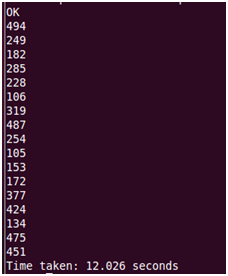
\includegraphics[width=0.8\textwidth]{photo/xjh1.png}
\caption{hive表的查询时间}
\end{minipage}
\hfill
\begin{minipage}[t]{0.45\linewidth}
\centering
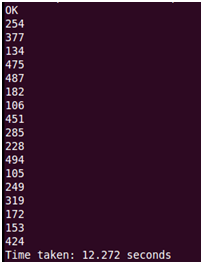
\includegraphics[width=0.8\textwidth]{photo/xjh2.png}
\caption{hive/hbase表的查询时间}
\end{minipage}
\end{figure}

\clearpage

\item
\begin{figure}[!ht]
\centering
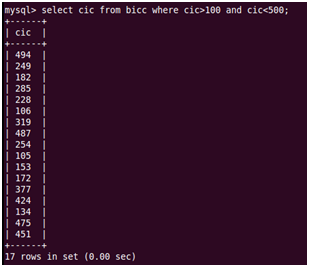
\includegraphics[scale=0.9]{photo/xjm1.png} 
\caption{mysql表的查询时间}
\end{figure} 

\item
\begin{figure}[!ht]
\centering
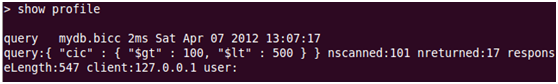
\includegraphics[]{photo/xjm2.png} 
\caption{mongoDB表的查询时间}
\end{figure} 
\end{description}

从这个实验得到的结果可以看出,hive和hive/hbase的结果是一个数量级,均在12s左右,而mysql和mongoDB所耗费的时间在一个数量级,差不多是3ms以下。他们之间的差别还是很大的。


第二个用到的测试用例是:
\begin{lstlisting}[language=SQL]
 select cic from bicc where cic<100 order by cic desc;
\end{lstlisting}

即从表bicc中挑出cic列值小于100的记录并且递减排序。这个查询最后得到的结果如图3-5到图3-8所示:
\begin{description}

\item
\begin{figure}[h]
\begin{minipage}[t]{0.45\linewidth}
\centering
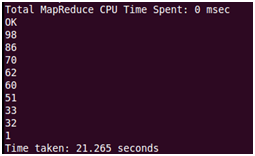
\includegraphics[width=0.8\textwidth]{photo/xjh3.png}
\caption{hive表的查询时间}
\end{minipage}
\hfill
\begin{minipage}[t]{0.45\linewidth}
\centering
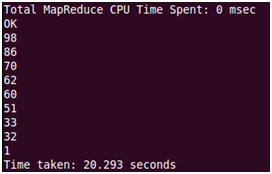
\includegraphics[width=0.8\textwidth]{photo/xjh4.png}
\caption{hive/hbase表的查询时间}
\end{minipage}
\end{figure}

\item
\begin{figure}[!ht]
\centering
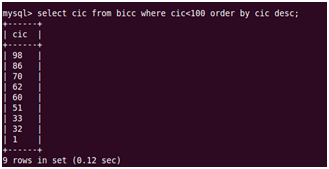
\includegraphics[]{photo/xjm3.png} 
\caption{mysql表的查询时间}
\end{figure} 

\item
\begin{figure}[!ht]
\centering
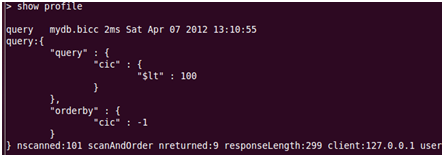
\includegraphics[]{photo/xjm4.png} 
\caption{mongoDB表的查询时间}
\end{figure} 

\end{description}
从第二个测试用例中得到的结果可以看出和由第一个测试用例得出的结果是一致的。

\subsection{大数量级}

  在小型数据级上做的实验放到大数据集上又会有不一样的结论。在原来基础上将实验用到的数据量加到很大,具体来说这里用到了已经建好的表yuyin,它拥有380万个记录,以及规模更大的表duanxin,它拥有940万个记录。同样也是采取两个测试用例加以互相验证,其中使用的第一个测试用例为:
\begin{lstlisting}[language=SQL]
select number from yuyin where ltype=4 and dtype=4;
\end{lstlisting}

这个语句很简单,实验的结果可以从图3-9到图3-12看出:
\clearpage
\begin{description}

\item
\begin{figure}[h]
\begin{minipage}[t]{0.4\linewidth}
\centering
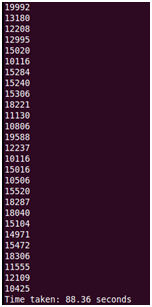
\includegraphics[width=0.7\textwidth,height=7cm]{photo/djh1.png}
\caption{hive表的查询时间}
\end{minipage}
\hfill
\begin{minipage}[t]{0.4\linewidth}
\centering
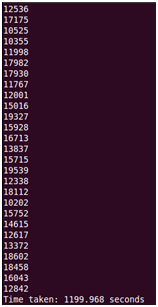
\includegraphics[width=0.7\textwidth,height=7cm]{photo/djh2.png}
\caption{hive/hbase表的查询时间}
\end{minipage}
\end{figure}

\item
\begin{figure}[!ht]
\centering
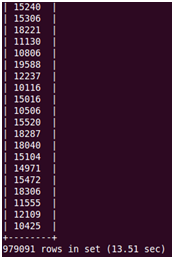
\includegraphics[]{photo/djm1.png} 
\caption{mysql表的查询时间}
\end{figure} 

\item
\begin{figure}[!ht]
\centering
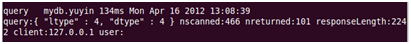
\includegraphics[scale=1.2]{photo/djm2.png} 
\caption{mongoDB表的查询时间}
\end{figure} 

\end{description}

从上面几个图中可以清晰的看到,hive查询用了88s,而hive/hbase查询足足用了1200s,mysql用了13s,mongoDB由于只查询头20条结果,因此时间不足一秒。可以看出hive相对来说较之前有所提升,而hive/hbase则相对下降,所花费的时间也达到了很难容忍的地步。为了对这个结果加以验证,我们又使用了第二个测试用例:
\begin{lstlisting}[language=SQL]
select distinct number from yuyin where duration<60 order by number desc;
\end{lstlisting}

实验的结果可以从图3-13到图3-16看出:
\begin{description}

\item
\begin{figure}[h]
\begin{minipage}[t]{0.4\linewidth}
\centering
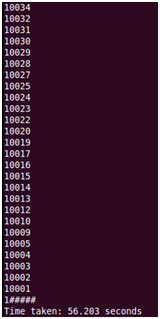
\includegraphics[width=0.7\textwidth,height=7cm]{photo/djh3.png}
\caption{hive表的查询时间}
\end{minipage}
\hfill
\begin{minipage}[t]{0.4\linewidth}
\centering
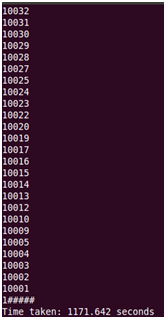
\includegraphics[width=0.7\textwidth,height=7cm]{photo/djh4.png}
\caption{hive/hbase表的查询时间}
\end{minipage}
\end{figure}

\item
\begin{figure}[!ht]
\centering
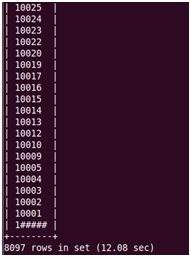
\includegraphics[]{photo/djm3.png} 
\caption{mysql表的查询时间}
\end{figure} 

\item
\begin{figure}[!ht]
\centering
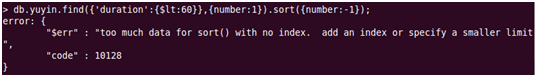
\includegraphics[]{photo/djm4.png} 
\caption{mongoDB表的查询时间}
\end{figure} 

\end{description}
从上面结果可以看出,hive用了56s,hive/hbase用了1171s,mysql用了12s,整体来说还是和第一个测试用例得到的结果是一致的。即时间hive/hbase>hive>mysql。

380万行的数据查询已经说明了一些问题,如果继续地增加数据量会有什么变化呢?接下来测试一下940万行的表duanxin,这里采用的测试用例为:
\begin{lstlisting}[language=SQL]
select distinct address from duanxin where mtype=0 and ltype=0;
\end{lstlisting}

实验的结果可以从图3-17到图3-19看出:
\begin{description}

\item
\begin{figure}[!ht]
\centering
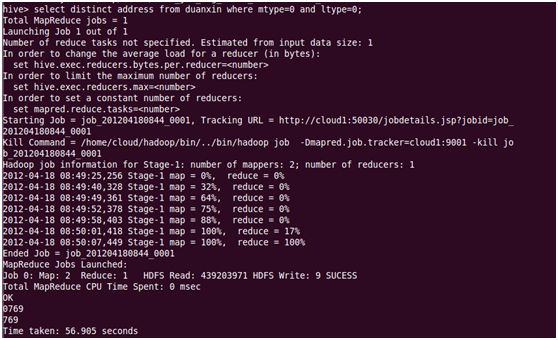
\includegraphics[scale=0.8]{photo/djh5.png}
\caption{hive表的查询时间}
\end{figure} 

\item
\begin{figure}[!ht]
\centering
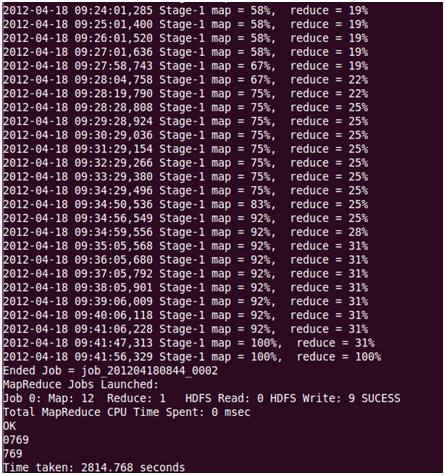
\includegraphics[scale=0.7]{photo/djh6.png}
\caption{hive/hbase表的查询时间}
\end{figure} 

\item
\begin{figure}[!ht]
\centering
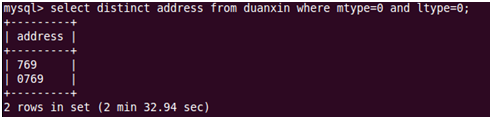
\includegraphics[]{photo/djm5.png} 
\caption{mysql表的查询时间}
\end{figure} 

\end{description}
从上三个图中可以看出,hive查询用了56秒,hive/hbase用了2814秒,mysql用了153秒。hive相对于mysql来说性能逐渐上升,到这时已经超出mysql达到最快,而hive/hbase这种方法的性能更加恶化,将近用了46分钟的时间,而hive花了不到一分钟。可想差别有多大。

\section{复杂查询}
复杂查询有很多种,比如嵌套查询等等。但最为典型的就是两个表之间的连接查询了。因此接下来的所有复杂查询都是指连接查询。而连接查询又分为很多种,如内连接,外连接等等。我们这里只考虑等值连接的情况。

\subsection{小数量级}
 由于表bicc和bssap表的结构相似,我们首先将这两个表进行等值连接。选取start\_time\_s这一项作为比较项。SQL语句为:
\begin{lstlisting}[language=SQL]
select distinct a.start_time_s join bssap b on a.start_time_s=b.start_time_s;
\end{lstlisting}

实验的结果可以从图3-20到图3-22看出:
\begin{description}

\item
\begin{figure}[h]
\begin{minipage}[t]{0.45\linewidth}
\centering
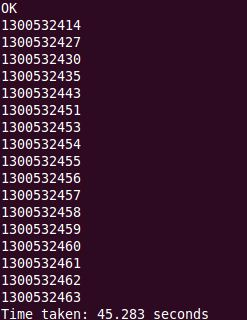
\includegraphics[width=0.8\textwidth,height=7cm]{photo/xfh1.png} 
\caption{hive表的查询时间}
\end{minipage}
\hfill
\begin{minipage}[t]{0.45\linewidth}
\centering
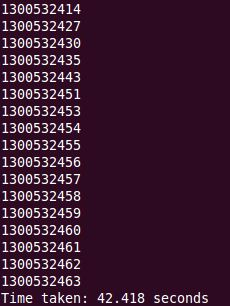
\includegraphics[width=0.8\textwidth,height=7cm]{photo/xfh2.png} 
\caption{hive/hbase表的查询时间}
\end{minipage}
\end{figure}

\item
\begin{figure}[!ht]
\centering
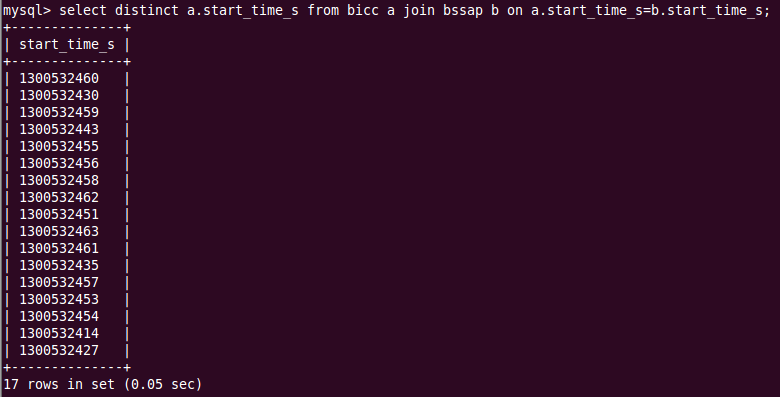
\includegraphics[width=0.8\linewidth]{photo/xfm1.png} 
\caption{mysql表的查询时间}
\end{figure} 

\end{description}
由于这两个表都非常小,join时花费的时间还是很少的。但仍然可以看出mysql远远快于hive和hive/hbase。

\subsection{大数量级}

将已经建好的表yuyin和表duanxin进行join等值连接:
\begin{lstlisting}[language=SQL]
select count(distinct a.address) from yuyin a join duanxin b on a.number=b.number;
\end{lstlisting}

由于表的规模太大,所以采用了让程序在服务器后台运行的方法。为了准确计算时间,我编写了shell脚本调用各个程序并计算调用程序前后的时间差,转换后的结果为秒。图3-23和3-24显示了hive和hive/hbase的脚本。

\begin{figure}[!ht]
\centering
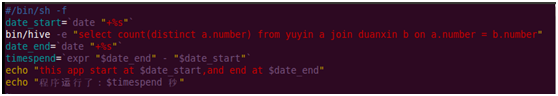
\includegraphics[]{photo/jb1.png} 
\caption{hive执行脚本}
\end{figure} 

\begin{figure}[!ht]
\centering
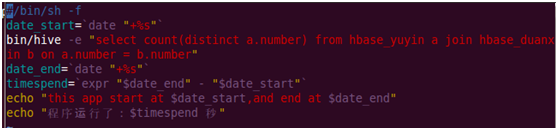
\includegraphics[]{photo/jb3.png} 
\caption{hive/hbase执行脚本}
\end{figure} 

后台执行脚本时输入:
\begin{lstlisting}[language=sh]
nohup ./h1.sh > h1out.txt 2>&1 &;
\end{lstlisting}
这样执行的结果就重定向到h1out.txt文本文件中。

mysql执行时也采取同样的办法。但是mysql第一次运行时出现“MySQL client ran out of memory”的错误。经过查阅资料,发现mysql分别使用mysql\_store\_result和mysql\_use\_result这两种方法存储结果集。mysql\_store\_result方法是把结果集全部存储在内存中,而mysql\_use\_result不把结果集存在客户端内存中,而是按需去mysql服务器取。由于这个连接查询结果集太大,如果用mysql\_store\_result的方法是放不下内存的,所以需要改用第二个方案。在执行时加入--quick选项。除此之外,由于结果太大,磁盘空间很可能不足,可以采用mysql提供的格式化结果的选项,使用grep命令只将带有时间的一行输出。

本次使用了count命令使得程序的输出没有受到磁盘空间的困扰,完整的mysql执行脚本为:
\begin{figure}[!ht]
\centering
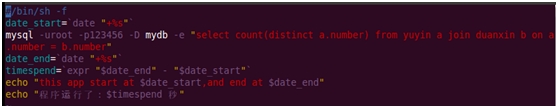
\includegraphics[]{photo/jb2.png} 
\caption{mysql执行脚本}
\end{figure} 



最后,实验的结果可以从图3-26到图3-28看出:
\begin{description}

\item
\begin{figure}[!ht]
\centering
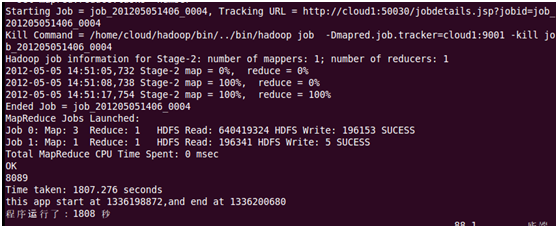
\includegraphics[]{photo/dfh1.png} 
\caption{hive表的查询时间}
\end{figure} 

\clearpage
\item
\begin{figure}[!ht]
\centering
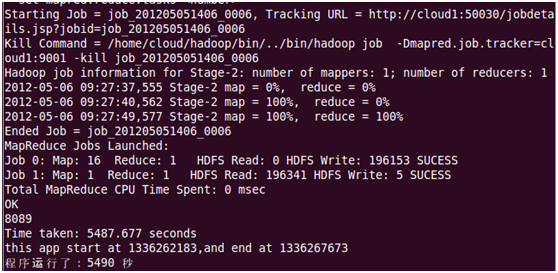
\includegraphics[]{photo/dfh2.png} 
\caption{hive/hbase表的查询时间}
\end{figure} 

\item
\begin{figure}[!ht]
\centering
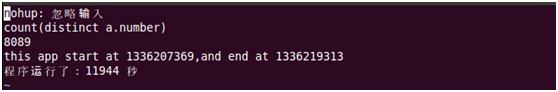
\includegraphics[]{photo/dfm1.png} 
\caption{mysql表的查询时间}
\end{figure} 

\end{description}
可以看出hive用了1808秒,hive/hbase用了5490秒,mysql用了11944秒。mysql执行的时间明显高于其他。

\section{总结}

\begin{table}[!h]
\arrayrulewidth=1pt
\centering
{\Large
\begin{tabular}{|c|c|c|c|}\hline
\rowcolor{gray!50} & hive & hive/hbase & mysql \\\hline
\rowcolor{green!60}简单查询(100行) & 12s-20s & 12s-20s & 0ms-100ms \\\hline
\rowcolor{green!20} 简单查询(380万行) & 88s & 1200s  & 14s \\\hline
\rowcolor{green!60} 简单查询(940万行) & 57s & 2814s & 153s \\\hline
\rowcolor{green!20} 复杂查询(小数量级) & 45s & 42s & 5ms \\\hline
\rowcolor{green!60} 复杂查询(大数量级) & 1808s & 5490s & 11944s \\\hline
\end{tabular}
}
\caption{实验数据汇总}
\end{table}

